\section{Электромагниты и постоянные магниты.}

\imc[1\textwidth]{82.png}

\[
\vec{B}_{\text{ж}}=\vec{H}_{\text{ж}}+4\pi\vec{M}_{\text{ж}} \text{ ,где  }
\vec{H}_{\text{ж}}-\text{размагничивающие поле. }
\]

\begin{gather*}
    \underset{L}{\oint}\vec{H}d\vec{l}=\frac{4\pi}{c}IN \\
    || \\
    \frac{B}{\mu}l_{\text{ж}}+Bl=\frac{4\pi}{c}IN \\
    B=\left( \frac{l_{\text{ж}}}{\mu}+l  \right)^{-1} \frac{4\pi}{c}IN= \frac{4\pi IN}{\left( \frac{l_{\text{ж}}}{\mu} +l \right)c} \\
\end{gather*}

Пусть сердечник феррамагнитный:

\begin{minipage}[c]{0.4\textwidth} % Левая часть: изображение
    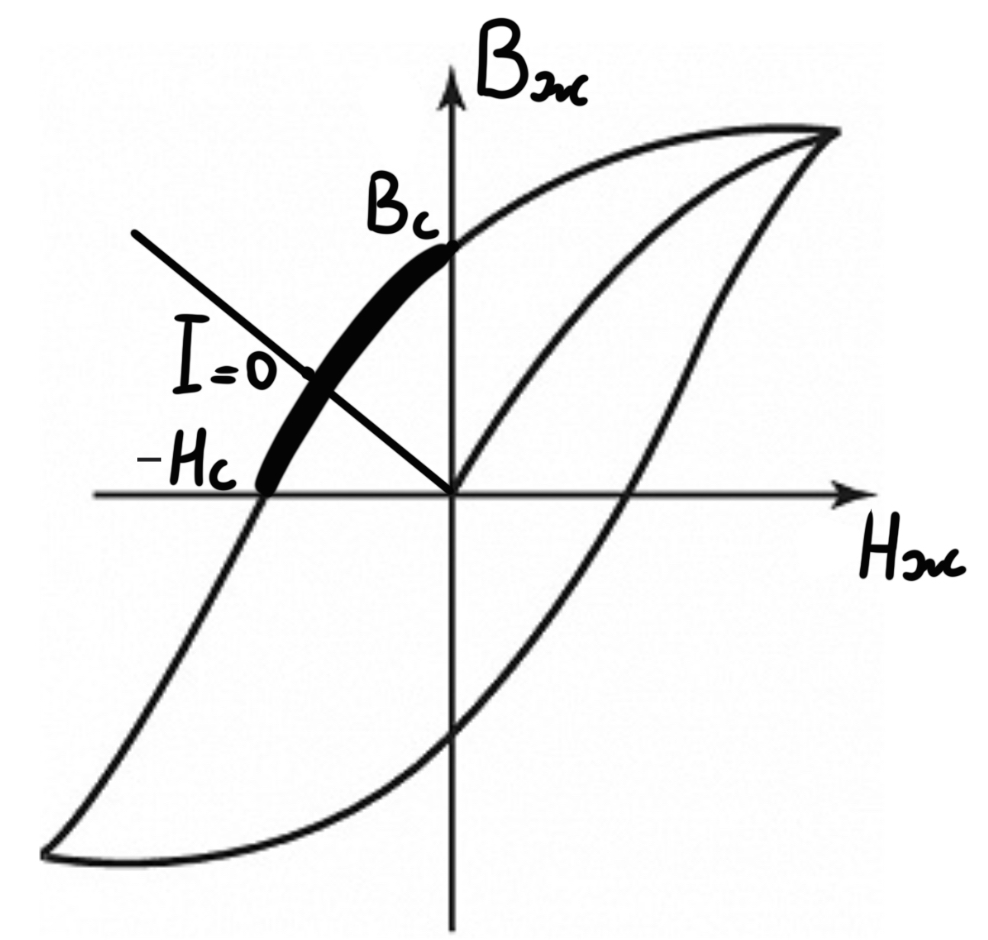
\includegraphics[width=\textwidth]{im/83.png} % Ваше изображение
\end{minipage}%
\hfill
\begin{minipage}[c]{0.6\textwidth} % Правая часть: текст
    \begin{gather*}
        H_{\text{ж}}l_{\text{ж}}+B_{\text{ж}}l=\frac{4\pi}{c}IN \text{ , пусть } I=0 \\
        B_{\text{ж}}=-H_{\text{ж}}\frac{l_{\text{ж}}}{l} \\
        B(H)=(H+H_c)\frac{B_c}{H_c} \\
        -H\frac{l_{\text{ж}}}{l}=(H+H_c)\frac{B_c}{H_c}     
    \end{gather*}
\end{minipage}
\[
H\left( \frac{l_{\text{ж}}}{l}-\frac{B_c}{H_c}  \right)=H_c \frac{B_c}{H_c}\Rightarrow \boxed{H=-B_c\left( \frac{l_{\text{ж}}}{l}+\frac{B_c}{H_c}  \right)^{-1} } 
\]

\[
B=B_c\left( \frac{l_{\text{ж}}}{l}+\frac{B_c}{H_c}  \right)^{-1}\frac{l_{\text{ж}}}{l} \Rightarrow \boxed{B=\frac{B_c}{1+\frac{B_cl}{H_cl_{\text{ж}}} }} 
\]

\begin{minipage}[c]{0.4\textwidth} % Левая часть: изображение
    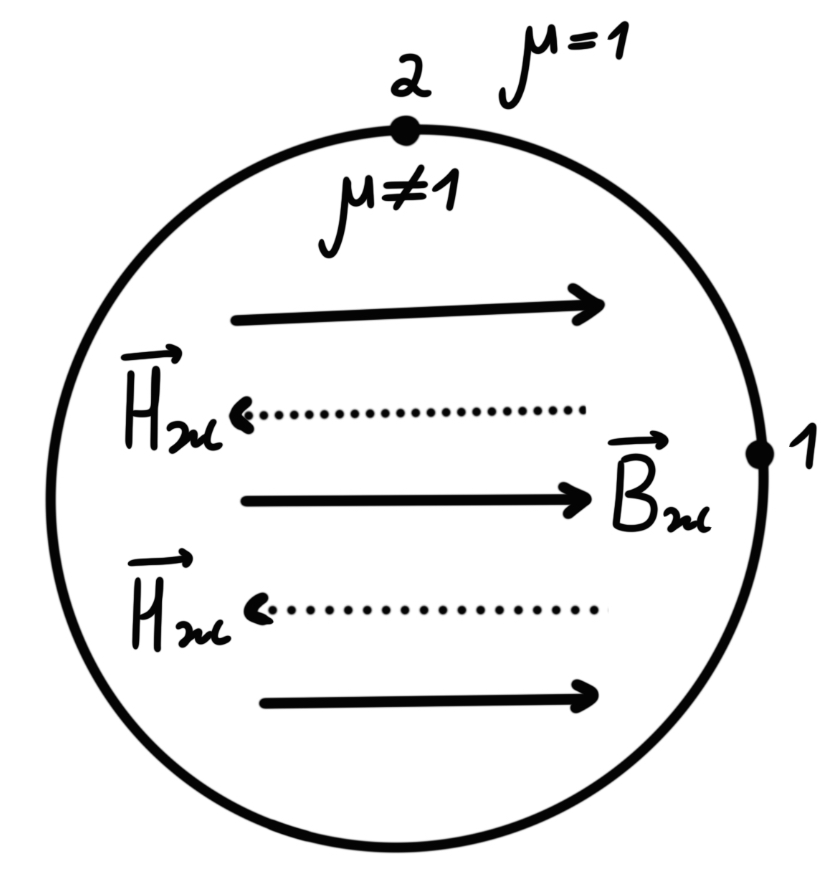
\includegraphics[width=\textwidth]{im/84.png}% Ваше изображение
\end{minipage}%
\hfill
\begin{minipage}[c]{0.6\textwidth} % Правая часть: текст
    Радиус окржности а.
    \begin{gather*}
        \vec{H}=-\frac{\vec{m}}{r^3}+3\frac{(\vec{m}\vec{r})\vec{r}}{r^5} \\
        \text{В точке }(1): B|_n-\text{непр. }: \\
        \vec{B}_{\text{ж}}=\frac{2}{a^3}\Rightarrow m=\frac{a^3B_{\text{ж}}}{2} \\
        \text{В точке }(2): H|_{\tau}-\text{ непр.}: \\
        H_{\text{ж}}=-\frac{m}{a^3} 
    \end{gather*}
\end{minipage}
\newpage
\[
\begin{array}{ccc}
m=\frac{4}{3}\pi a^3M_{\text{ж}} & & B_{\text{ж}}=H_{\text{ж}}+4\pi M_{\text{ж}} \\
\Downarrow & & \Downarrow \\
\frac{a^3B_{\text{ж}}}{2}=\frac{4}{3}\pi a^3M_{\text{ж}} & \Rightarrow & H_{\text{ж}}=4\pi M_{\text{ж}}-B_{\text{ж}}= \\
\end{array}
\]

\[
=4\pi M_{\text{ж}}-\frac{8}{3}\pi M_{\text{ж}}=\frac{4}{3}\pi M_{\text{ж}}  
\]

\[
H_{\text{ж}}=-\frac{4}{3}\pi M_{\text{ж}}=N M_{\text{ж}}
\]

\[
\text{Где }N\text{-размагничивающий  фактор}
\]